%\documentclass{article}
%\usepackage{graphicx,subfigure}
%\begin{document}

\begin{figure}[h]
  \centering
   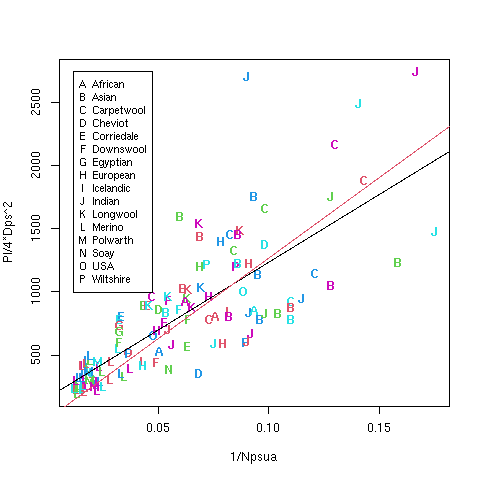
\includegraphics[width=0.9\textwidth]{cartercsax1ovnreg.png}
  \caption{Plot of breed means for reciprocal of follicle density and fibre cross sectional area from Carter(1968)~\cite{cart:68}. The black line is a linear regression fitted with an intercept. The red line is a linear regression fitted without an intercept.}
  \label{fig:carternxc}
\end{figure}

%\end{document}

